\section{Metodologia}

\subsection{Protocolo}

O protocolo utilizado foi baseado na metodologia de Amplificação-Mutação-Seleção "AMS" (figura \ref{fig:fluxograma-principal}) onde os processos de amplificação e mutação eram representados pelo PCR e a seleção era representada pelo próprio SELEX que buscava sequências de afinidade. Os códigos foram desenvolvidos em Python por questão de facilidade em
tratamento de “strings”, pois eram assim que as moléculas eram representadas, outra questão era a facilidade em desenvolver gráficos para o fácil entendimento e comportamento das moléculas.

\begin{figure}[!h]
    \centering
    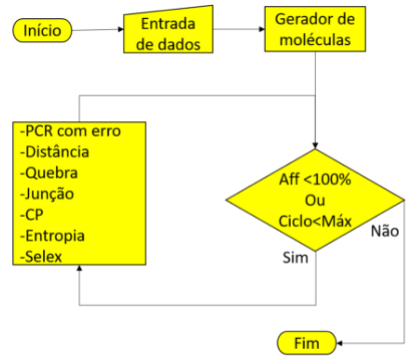
\includegraphics[width=10cm]{figures/img-fluxo1.png}
    \caption{Fluxograma principal}
    \label{fig:fluxograma-principal}
\end{figure}

As primeiras etapas do ciclo eram amplificação e mutação, etapas essas que eram
feitas em somente um passo. O PCR com erro (PCR error prone) era processo que
realizava as replicações, colocando assim, uma molécula sucessora que nessa pesquisa
vai ser chamada de molécula-filha. Essa molécula-filha pode conter pequenos erros no
seu código que podem simplesmente favorecer ou prejudicar ela na seleção natural.

A etapa que diz respeito sobre a distância foi utilizada para análise de cada
molécula, pois com ela era possível saber a quantidade de bases que mudaram após a sua 
12
replicação, o método usado para o tamanho constante foi a distância de Hamming e para
as moléculas com tamanhos variados a distância de Levenshtein.

Em dois dos três cenários foram implementados métodos para a variação de
tamanho, métodos esses que podiam tanto aumentar uma molécula quanto diminuir a
mesma, trazendo assim, um modelo mais real e mais complicado pois ajustar esses dois
processos emanaram muitos esforços e tentativas com intenção de equilibrar este
processo.

O método de Monte Carlo chamado de Constant Population (CP) foi um algoritmo
muito importante para a análise das moléculas pois sem ele as replicações iriam tomar
uma proporção enorme em questão a quantidade de moléculas, com ele foi possível
colocar um limite máximo na quantidade de moléculas.

A função da entropia foi medir o grau de desordem das moléculas no ciclo em bits
e ver o comportamento do resultado da entropia no gráfico, sendo ele, 2 que seria o maior
grau de aleatoriedade por existirem somente 4 bases e 0 caso todas moléculas fossem
exatamente iguais que é um fato impossível de acontecer.

A terceira etapa do ciclo foi a seleção que mimetizava o próprio SELEX. Foi
escolhido uma sequência de bases que caracterizava a afinidade e se a molécula era “apta”
ou não a seleção, na pesquisa essa sequência de bases são chamadas de sequencias afins,
conservadas, alvos ou filtro. A intenção das sequências é mimetizar um vírus ou proteína
e ver o quão forte ela é na seleção natural.


\subsection{Código}

O fluxo do programa desenvolvido para os cenários 1, 2 e 3 estão representados nas figuras abaixo:

\begin{figure}[!h]
    \centering
    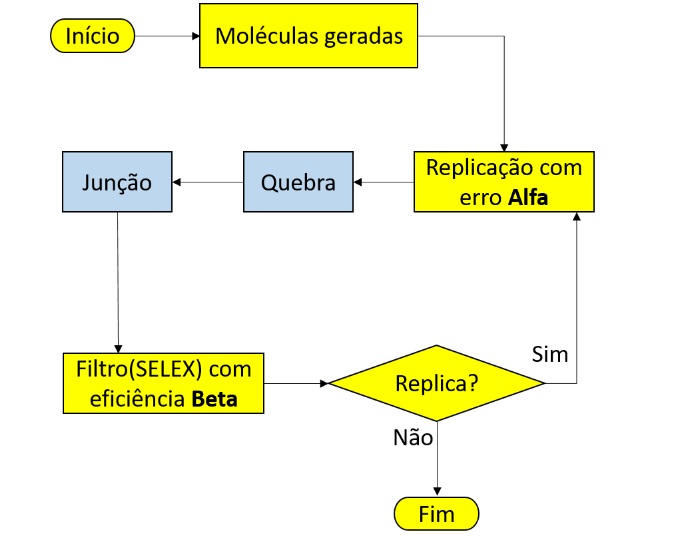
\includegraphics[width=10cm]{figures/img-fluxo2.png}
    \caption{Fluxograma das simulações dos cenários 1 e 2.}
    \label{fig:fluxograma-cen1-cen2}
\end{figure}

\newpage

\begin{figure}[!h]
    \centering
    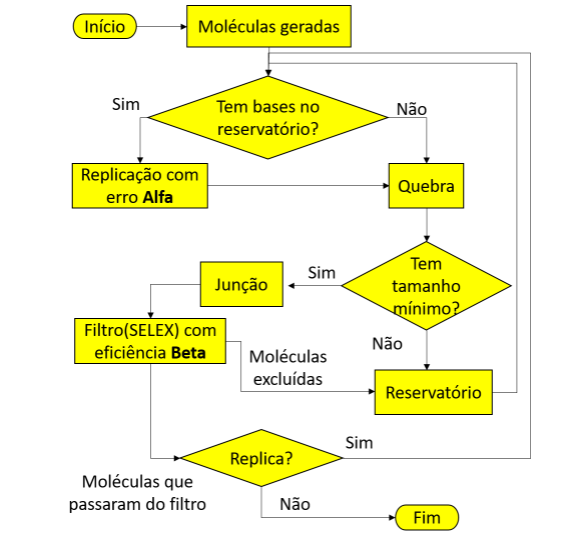
\includegraphics[width=14cm]{figures/img-fluxo3.png}
    \caption{Fluxograma da simulação do cenário 3.}
    \label{fig:fluxograma-cen3}
\end{figure}

O código foi desenvolvido em Python e contém 5 classes. Sendo elas:\\
\textbf{Class\_RNA.py}, \textbf{Class\_Filtro.py}, \textbf{Class\_Equação.py}, \textbf{Class\_Entropia.py} e
\textbf{Class\_Distancia.py}. Todas as 5 classes são chamadas em um código principal que chama a função a cada ciclo e após o término da simulação é gerado quatro gráficos, sendo eles: Afinidade x Ciclo, Entropia x Ciclo, Quantidade de moléculas x Ciclo, Tamanho médio x Ciclo. O código principal também é capaz de gerar o desvio padrão, a
variância, tamanho da menor e maior molécula e por fim mostrar os pontos de máximo e mínimo da afinidade.

A classe RNA faz todo o processo de \emph{Amplificação e Mutação}. É responsável pela
maior parte do processo tendo funções que fazem as seguintes operações: Gera a
quantidade de moléculas desejadas com o tamanho desejado para a primeira geração de
moléculas entrar no ciclo; faz a replicação com erro \textbf{Alfa}, sendo esse erro aplicado base
a base em cada molécula; limita a quantidade de moléculas com o método de Monte Carlo
chamado Constant Population (CP) que exclui moléculas aleatoriamente, assim, não
influenciando muito no resultado e mantendo a quantidade de moléculas em uma
quantidade desejável, o método foi que adaptado para deletar aleatoriamente metade das
moléculas afins e metade das moléculas não-afins reduzindo o erro a zero. Como essa
classe fala de tudo que diz respeito a estrutura da molécula nada mais justo do que colocar
as funções de quebra e junção nessa classe. O processo de quebra e junção só foram
implementados nos cenários 1 e 2, no caso da junção, foi desenvolvida escolhendo uma
sequência de 5 bases que caso a molécula tivesse no seu \emph{códon} teria uma porcentagem de
chance de junção com uma molécula afim, no cenário 2 essa porcentagem foi de 100\%,
já no cenário 3 foi de 10\%. No processo de quebra foi escolhido uma sequência de 3 bases
que se caso uma molécula tivesse no seu códon essa molécula ela se quebrava logo após,
a chance de quebra foram as mesmas, 100\% no cenário 2 e 10\% no cenário 3.

A classe Distância é responsável por parte da análise das moléculas, é com ela que
analisamos uma molécula e a sua duplicata ou molécula-filha sendo colocada uma
embaixo da outra e olhando base por base, caso tenha diferença é incrementado 1 na
contagem da distância dessa molécula-filha. Esse processo é feito a cada alteração na
molécula sendo ela replicação, quebra, junção ou filtragem para que se tenha total
controle da molécula. Vale lembrar que a distância usada no primeiro cenário é a distância
de Hamming pois as moléculas têm o mesmo tamanho e no segundo e terceiro cenário é
usado a distância de Levenshtein pois tem tamanhos variados ao decorrer dos ciclos.

A classe Entropia foi responsável pelo cálculo da entropia de Shannon no
primeiro cenário como teve tamanho médio das moléculas sempre constante, foi exato o
valor da medida. O cenário 2 e 3 teve um grau de entropia aproximado por conta dos
tamanhos variados, por conta disso foi escolhido pelo menor tamanho que uma molécula
poderia ter, que no caso desses cenários o tamanho mínimo era 10, foi testado também
pegando como referência a menor molécula do ciclo, mas graficamente os valores se
mostravam com enormes saltos.

A classe Filtro seria o próprio SELEX, onde moléculas afins tinham vantagens
sobre as não-afins, no cenário 1 e 2 a probabilidade de as moléculas afins saírem é de 0\%
já no cenário 3 é de 5\%. Com exceção do cenário 1, os outros cenários contêm filtragem
por distância da molécula replicada com a original, ou seja, caso uma molécula-filha tenha

10\% de diferença da sua descendente, ela tem 10\% de chance morrer. A eficiência \textbf{Beta}
se refere a probabilidade que uma molécula não-afim sobreviver ao filtro. Lembrando que
para sabe o valor da afinidade foi executada a equação \ref{equation-mols}:

\begin{equation}
    \label{equation-mols}
    Aff = \frac{\text{Mol. afins}}{\text{Total de moléculas}}
\end{equation}

A classe Equação tem o intuito de trazer uma equação modelada para o cenário 1
com intenção de mostrar os resultados do método calculado e simulado para uma
comparação entre quantidade de moléculas e eficiência de filtro trazendo assim uma
segurança maior quanto aos resultados exibidos.

